\chapter{Advanced Models}

Stimulated by the surge in data availability and advancements in computational power, alongside the growing popularity of advanced machine learning models, financial institutions are increasingly motivated to leverage advanced models for predicting the probability of default. The objectives include enhancing model performance and uncovering previously unseen interactions among risk factors. However, challenges such as limited transparency in explaining individual predictions and constraints imposed by regulatory requirements and data protection laws, as discussed in Chapter \ref{sec:ref_leg}, force financial institutions to be hesitant to implement these algorithms in the calculation of regulatory capital. \cite[p. 4]{EBA:2023}

These advanced models can be broadly classified into three categories \cite[p. 43-45]{Roberts2022}:

\begin{enumerate}
  \item Supervised Learning: In this category, a target variable is provided and utilized during the training process. Boosting methods are employed to improve the classification of misidentified observations. Decision Trees and Random Forests are prominent examples.
\item Unsupervised Learning: Here, unlabeled data is used for training, relying solely on features to uncover underlying patterns or relationships within the data without explicit guidance. Examples include the kNN algorithm and Clustering.
\item Unsupervised Learning: In this paradigm, an "agent" learns to make decisions by interacting with an environment. It receives feedback in the form of rewards or punishments based on the actions it takes, allowing it to learn the optimal strategy to maximize cumulative rewards over time.
\end{enumerate}

\section{Decision Trees}
\label{sec:dectrees}
Classification trees are used to separate the categories (default, non-default) as best as possible using explanatory factors. The split is determined by maximizing the homogeneity of the resulting subgroups, so-called branches. The algorithm calculates the measure for each possible threshold for numeric variables, while for categorical variables, it determines it for each unique value. This step is repeated until a stopping condition is met and the final subgroup is called a leaf. To avoid overfitting, the Decision Tree may be "pruned", where some branches are removed. The preliminary decision tree is applied on a separate data set, i.e., the validation sample, and to improve its performance, redundant splits are cut off. An example of a decision tree and the pruning process is visible in Figure \ref{fig:ml_dectree}. A Separate validation should then be performed on a third data set since the validation sample became part of the modeling process. 

\begin{figure}[H]
	\centering
	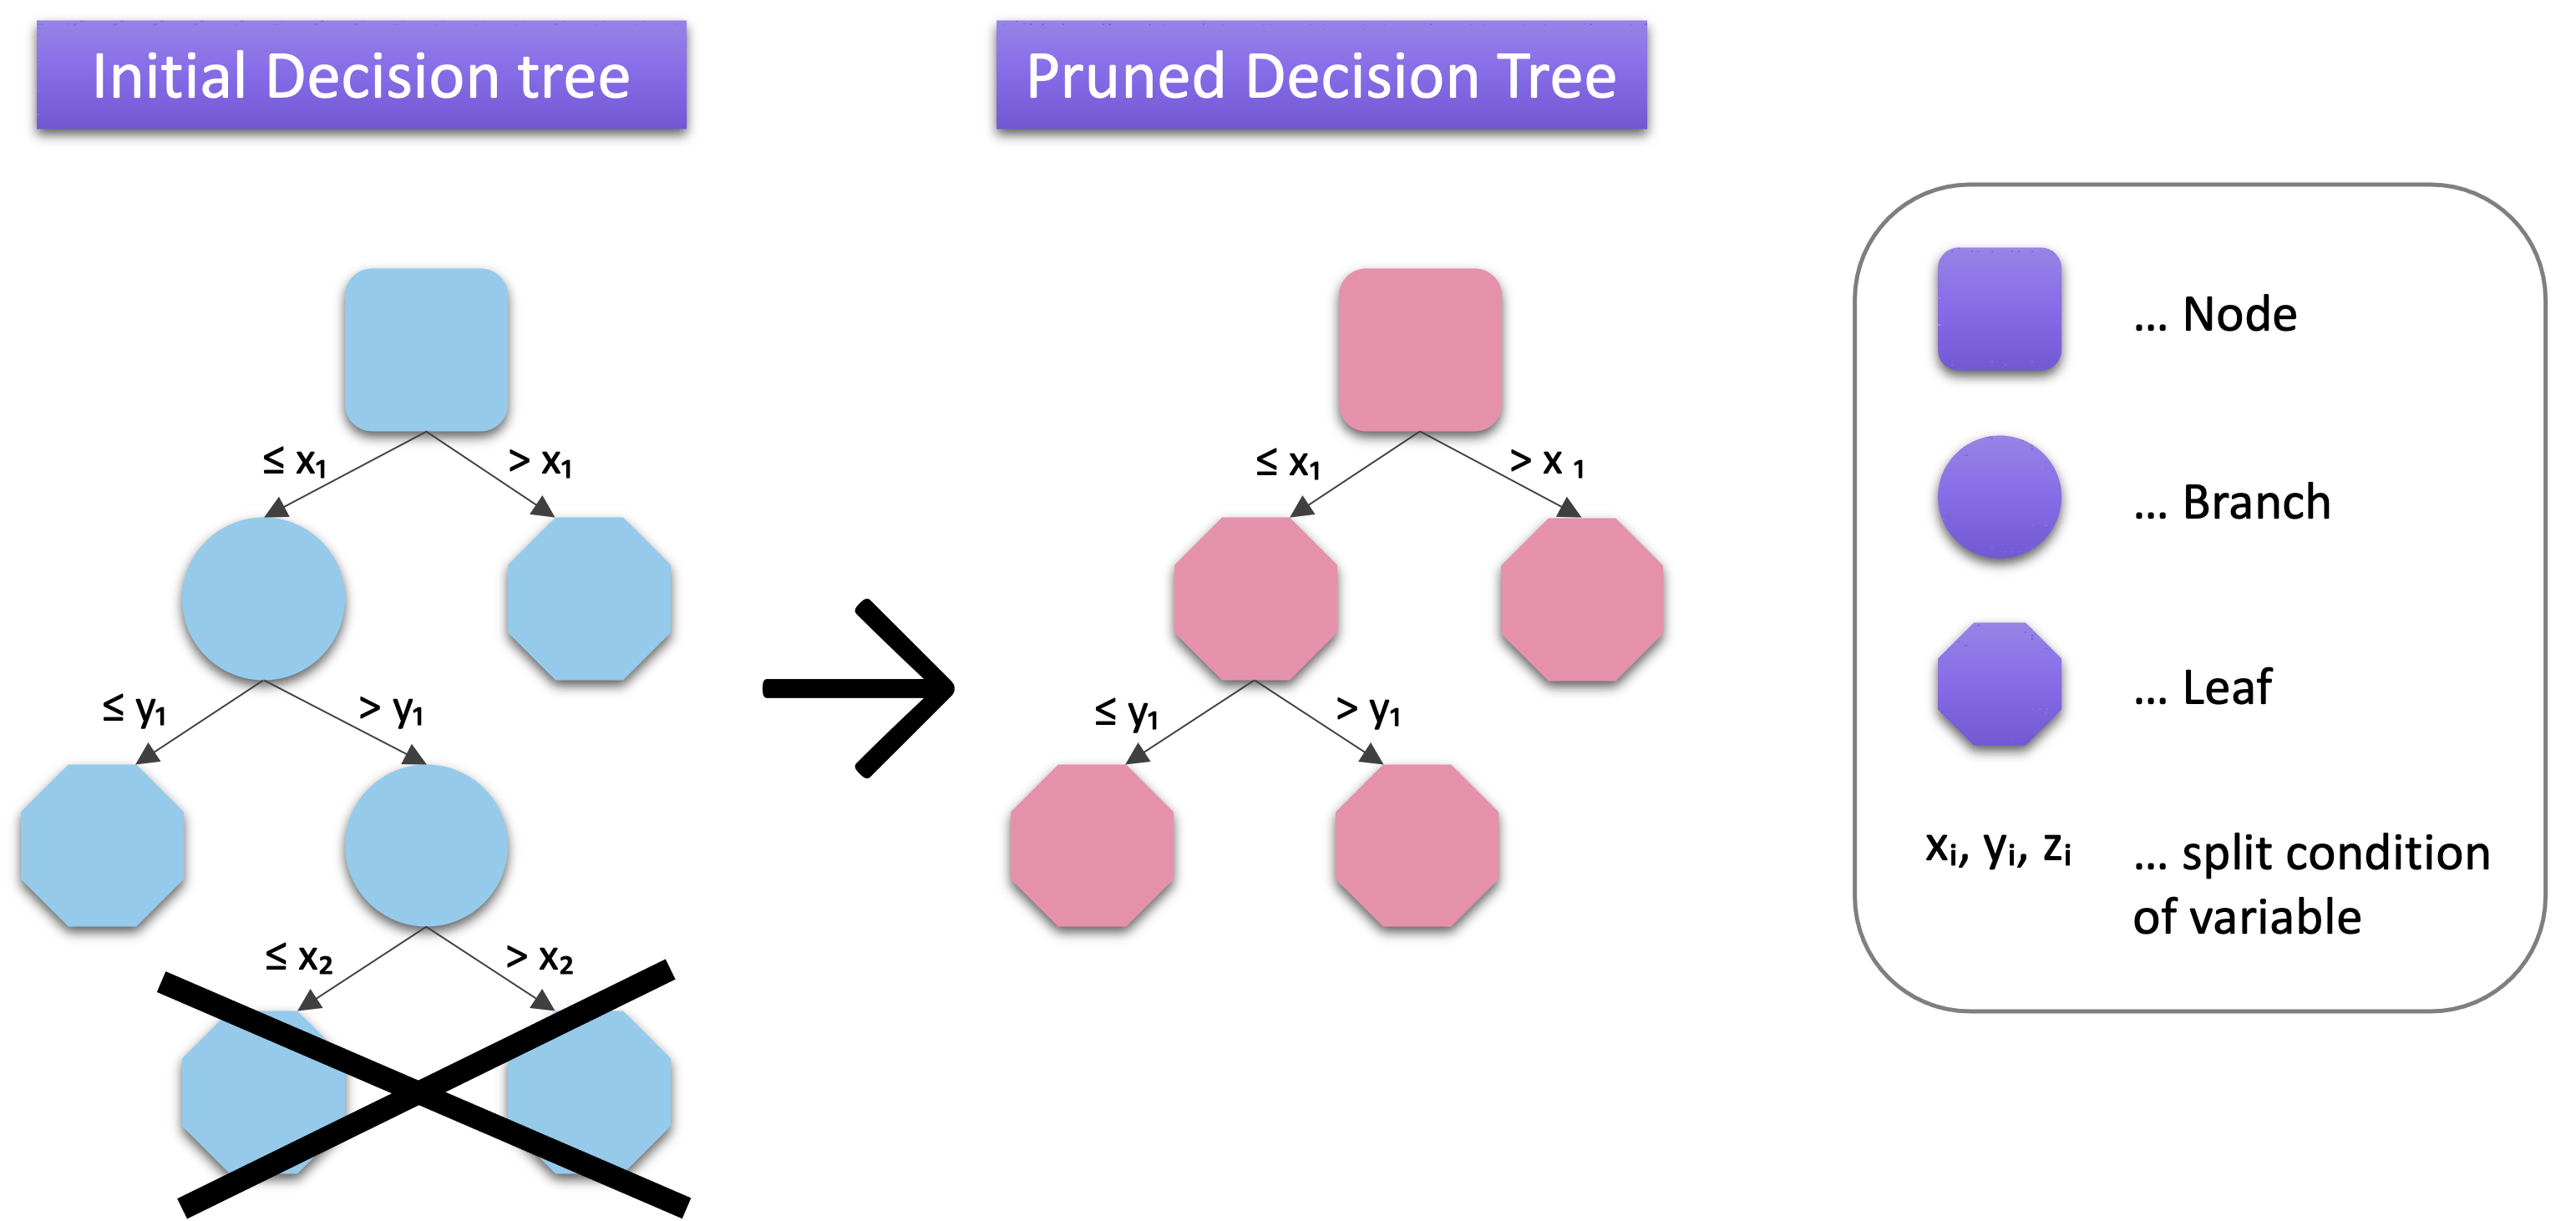
\includegraphics[width=0.625\textwidth]{./ML__DecTree.png}
    \caption{Decision Tree incl. Pruning}
    \label{fig:ml_dectree}
\end{figure}

The estimated PD is the average default rate per leaf and each terminal node can be classified into default or non-default class using a defined threshold. Popular statistics to measure homogeneity are the Gini index and Entropy index. The Gini index assumes a value between 0 and 1, where 0 means complete purity, 0.5 represents an equal distribution of all classes and 1 shows a random distribution across all classes. The formula is given in \ref{eq:ml_gini}. Decision trees usually perform worse than logistic regression models and are rather used to assess the best variables or segmentation possibilities. \cite[pp.~75-76]{Witzany:2017}

\begin{equation}
GINI = \sum_{i=1}^{n}  p_i \times (1 - p_i) \label{eq:ml_gini}
\end{equation}
where:
\begin{conditions}
 n  	& number of unique classes in variable \\
 p_{i}  & proportion of observations in class n
\end{conditions}

\subsection{Boosted Decision Trees and Random Forests} 
Boosted Decision Trees (BDT) or Gradient Boosted Decision Trees combine decision trees with boosting techniques to achieve higher predictive performance. This algorithm iteratively builds decision trees, placing more weight on misclassified observations in each iteration, resulting in a better model. BDT can capture complex interactions and non-linear relationships in PD modeling. 

Random forests are an ensemble learning method that combines multiple decision trees to make predictions. However, unlike boosted decision trees, random forests build each tree independently, without sequential corrections (Figure \ref{fig:ml_ranforest}). This approach reduces the risk of overfitting and the variance of predictions. Random forests are known for their robustness, scalability and ability to handle high-dimensional data. \cite[p.~88]{Witzany:2017}

\begin{figure}[H]
	\centering
	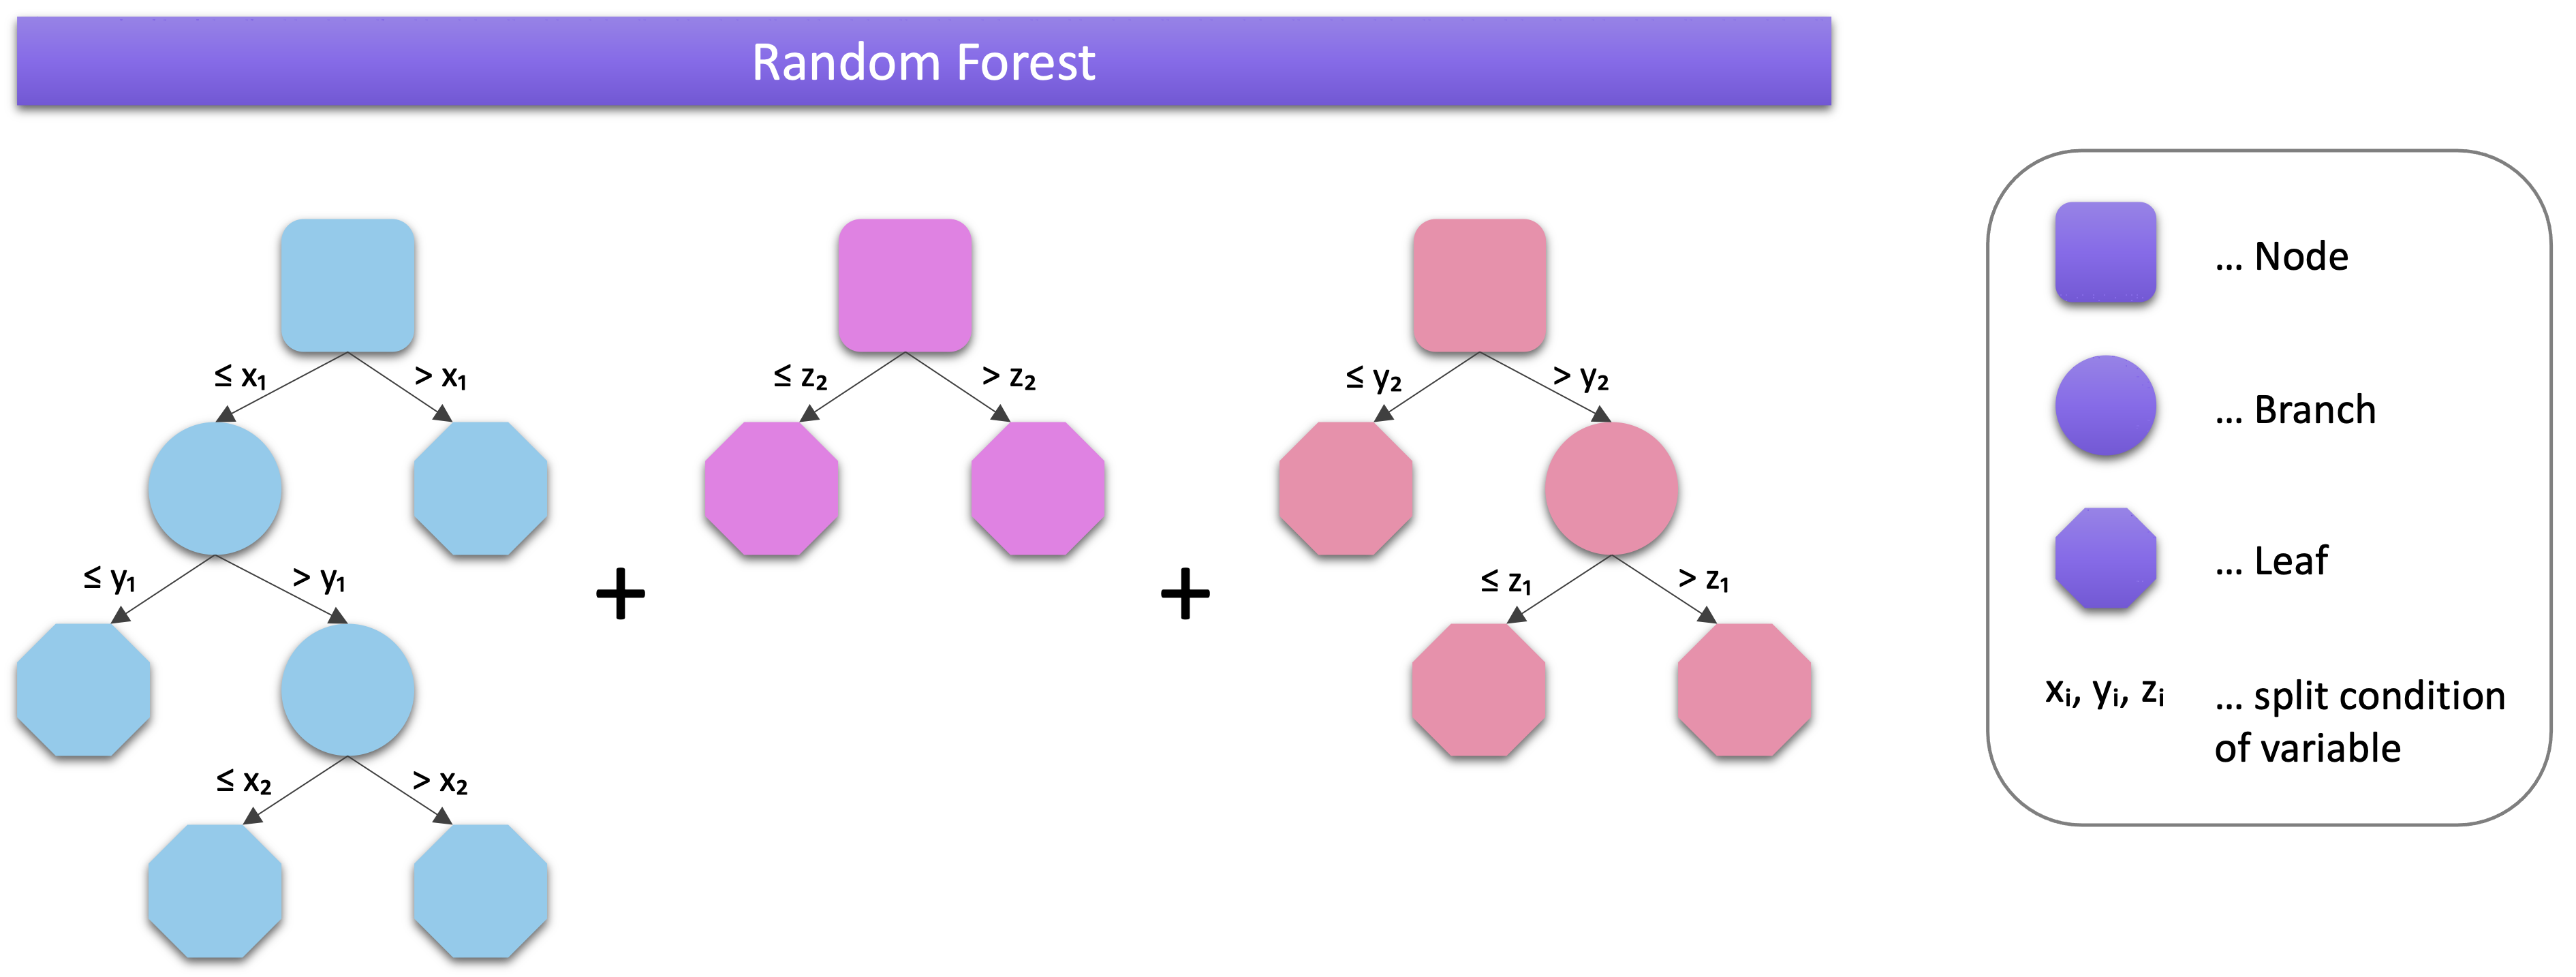
\includegraphics[width=0.625\textwidth]{./ML__Random_forest.png}
    \caption{Random Forest}
    \label{fig:ml_ranforest}
\end{figure}

\section{Other Models}

\subsection{Neural Networks}
Neural networks, inspired by the structure and function of the human brain, can learn intricate patterns and nonlinear relationships in data. They consist of multiple layers of interconnected nodes, also called neurons, where each neuron is assigned a simple computation and uses activation functions to pass along a value. The result of the model is a numerical or classification value. Commonly used activation functions are logistic, threshold and tangent hyperbolic functions.

The initial layer is referred to as the input layer, the final layer as the output layer and those in-between are known as hidden layers. An illustration is visible in Figure \ref{fig:ml_neurnet}. Due to the virtually endless possibility of configurations, there is a possibility of over-parametrization, especially with an increasing number of hidden layers and nodes, also called deep neural networks. \cite[pp.~79-80]{Witzany:2017}

\begin{figure}[H]
	\centering
	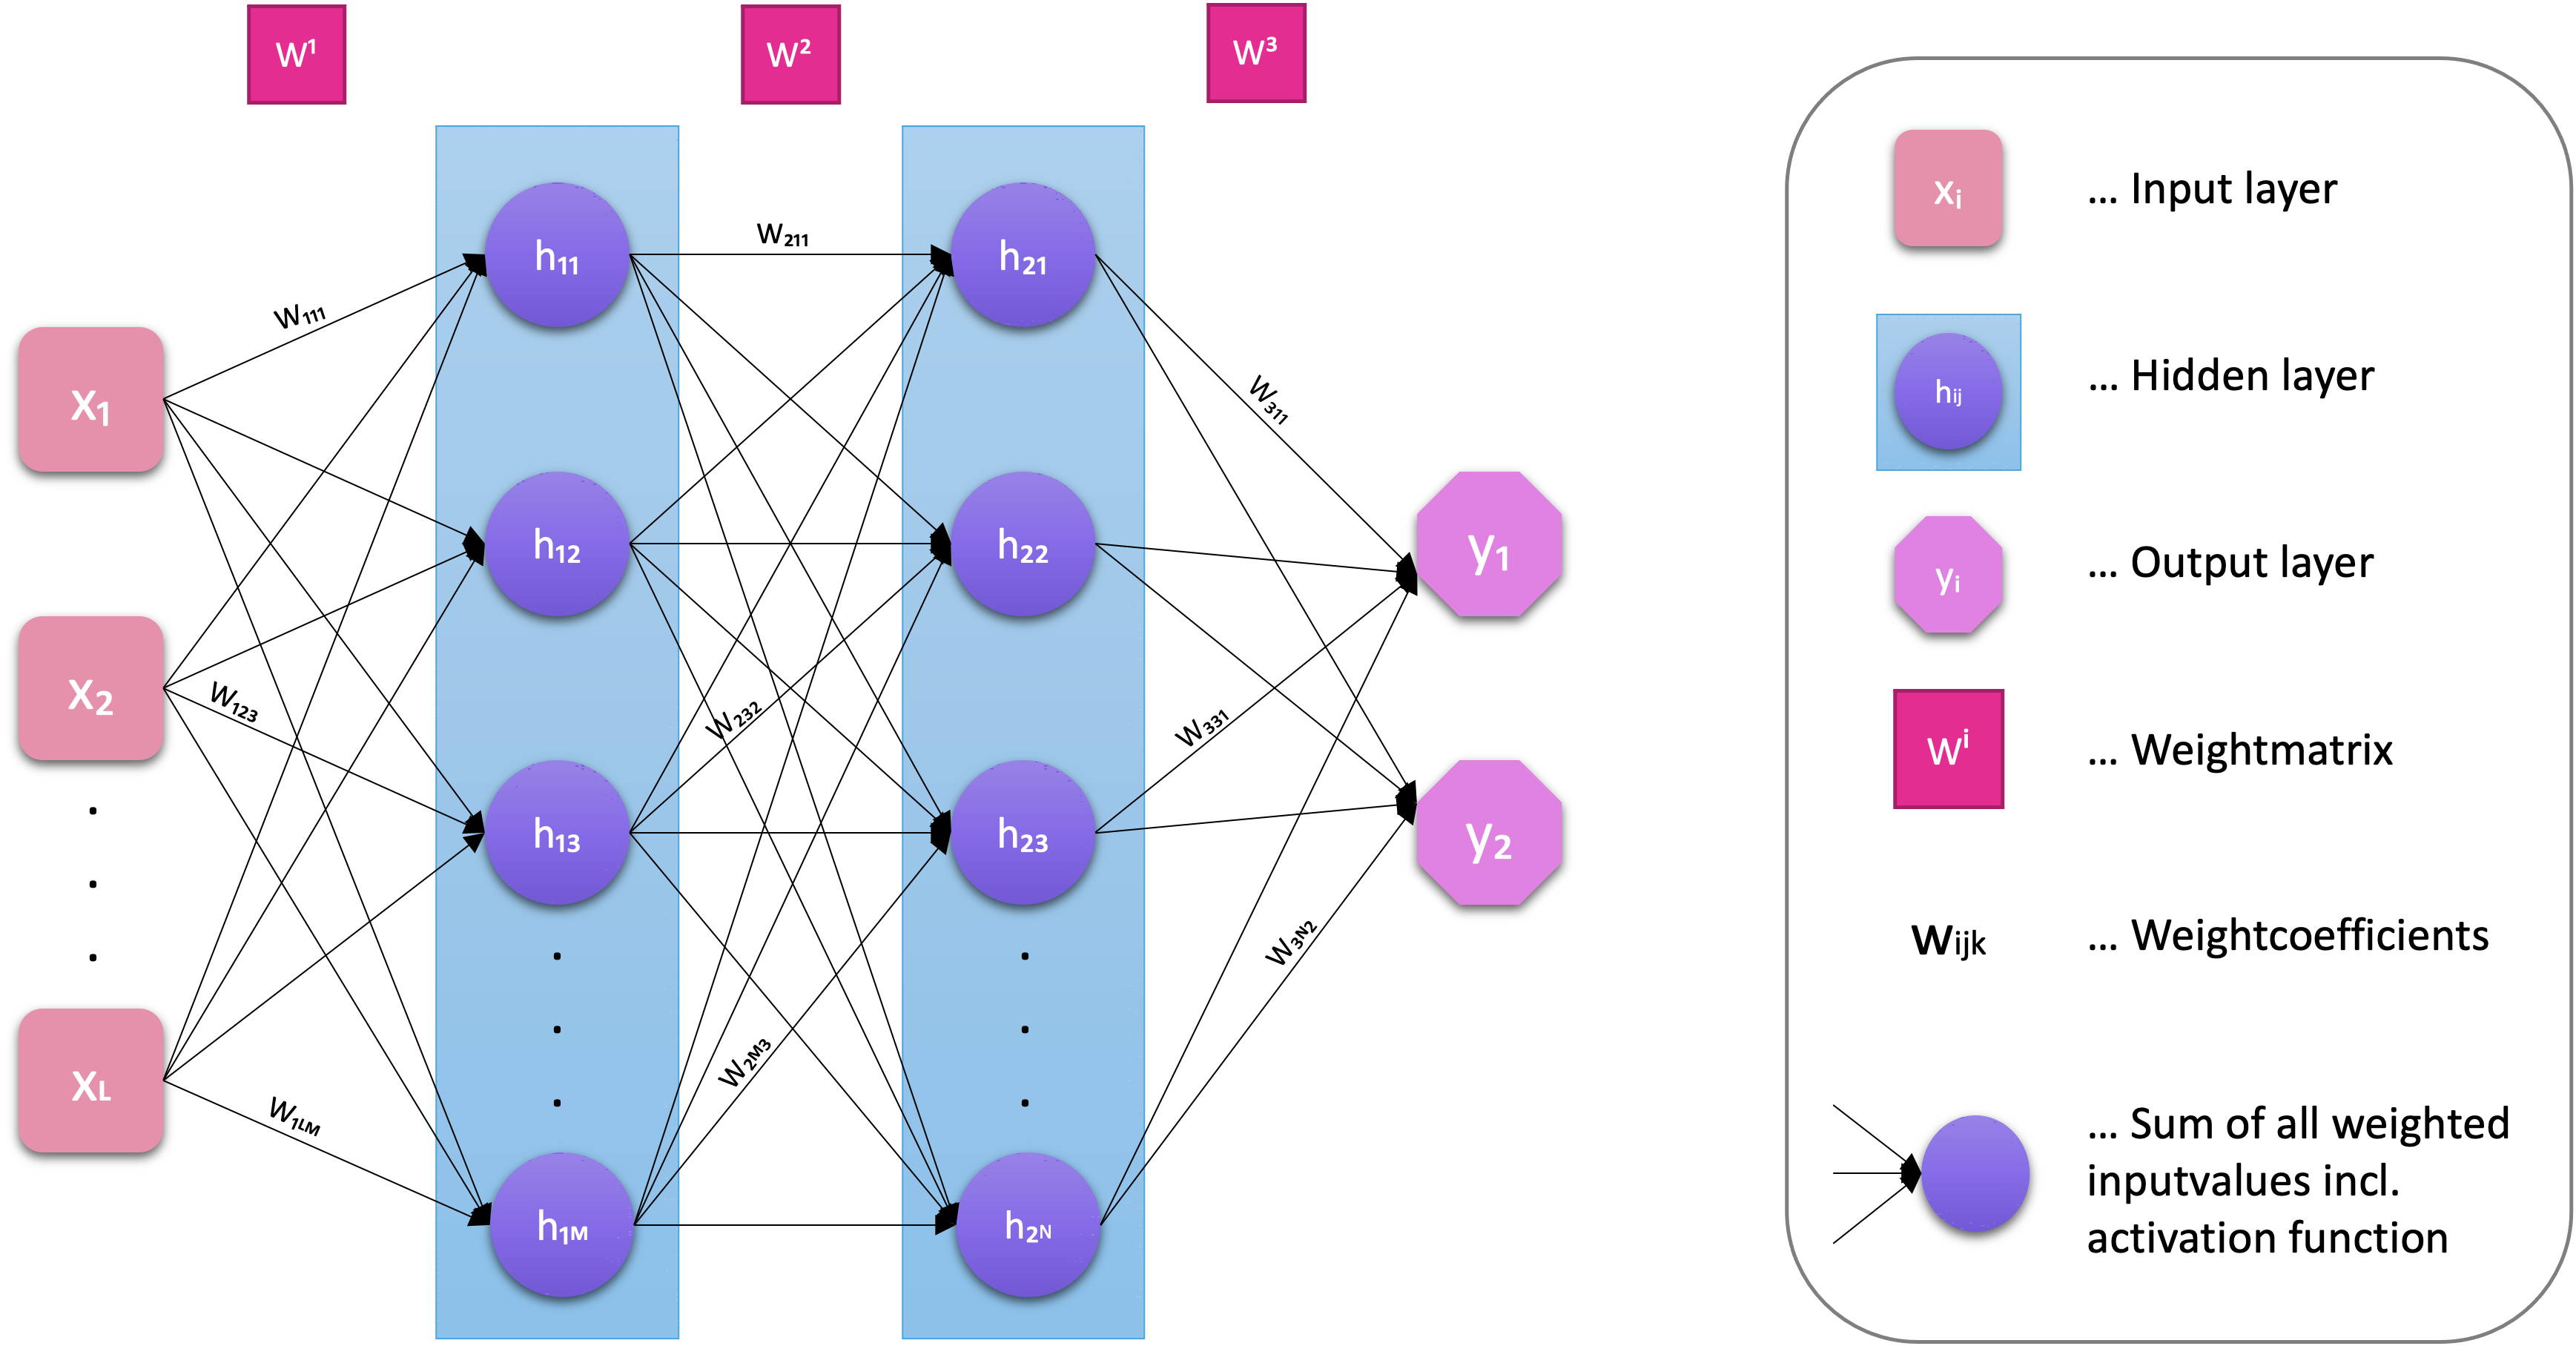
\includegraphics[width=0.625\textwidth]{./ML__MLP.png}
    \caption{Neural Network}
    \label{fig:ml_neurnet}
\end{figure}

\subsection{k-Nearest Neighbour}
\label{sec:kNN}
Based on a data set with explanatory factors and observed default events, the unknown PD of a new data entry can be estimated by taking the nearest data points determined via their risk factors and calculating the average default rate of the new data point. The Euclidean metric or Manhattan Distance can be used: The Euclidean distance measures the straight-line distance between two points. In comparison, the Manhattan distance is the sum of the absolute differences between two points in a space, where it can only move along coordinate axes. The number of nearest neighbors "k" is a hyper-parameter. The advantages of this model are the simple approach and the possibility to update new and outdated data entries dynamically and if k is set as a low number, a credit analyst can view individual scorings manually. \cite[p.~83]{Witzany:2017}

\begin{figure}[H]
	\centering
	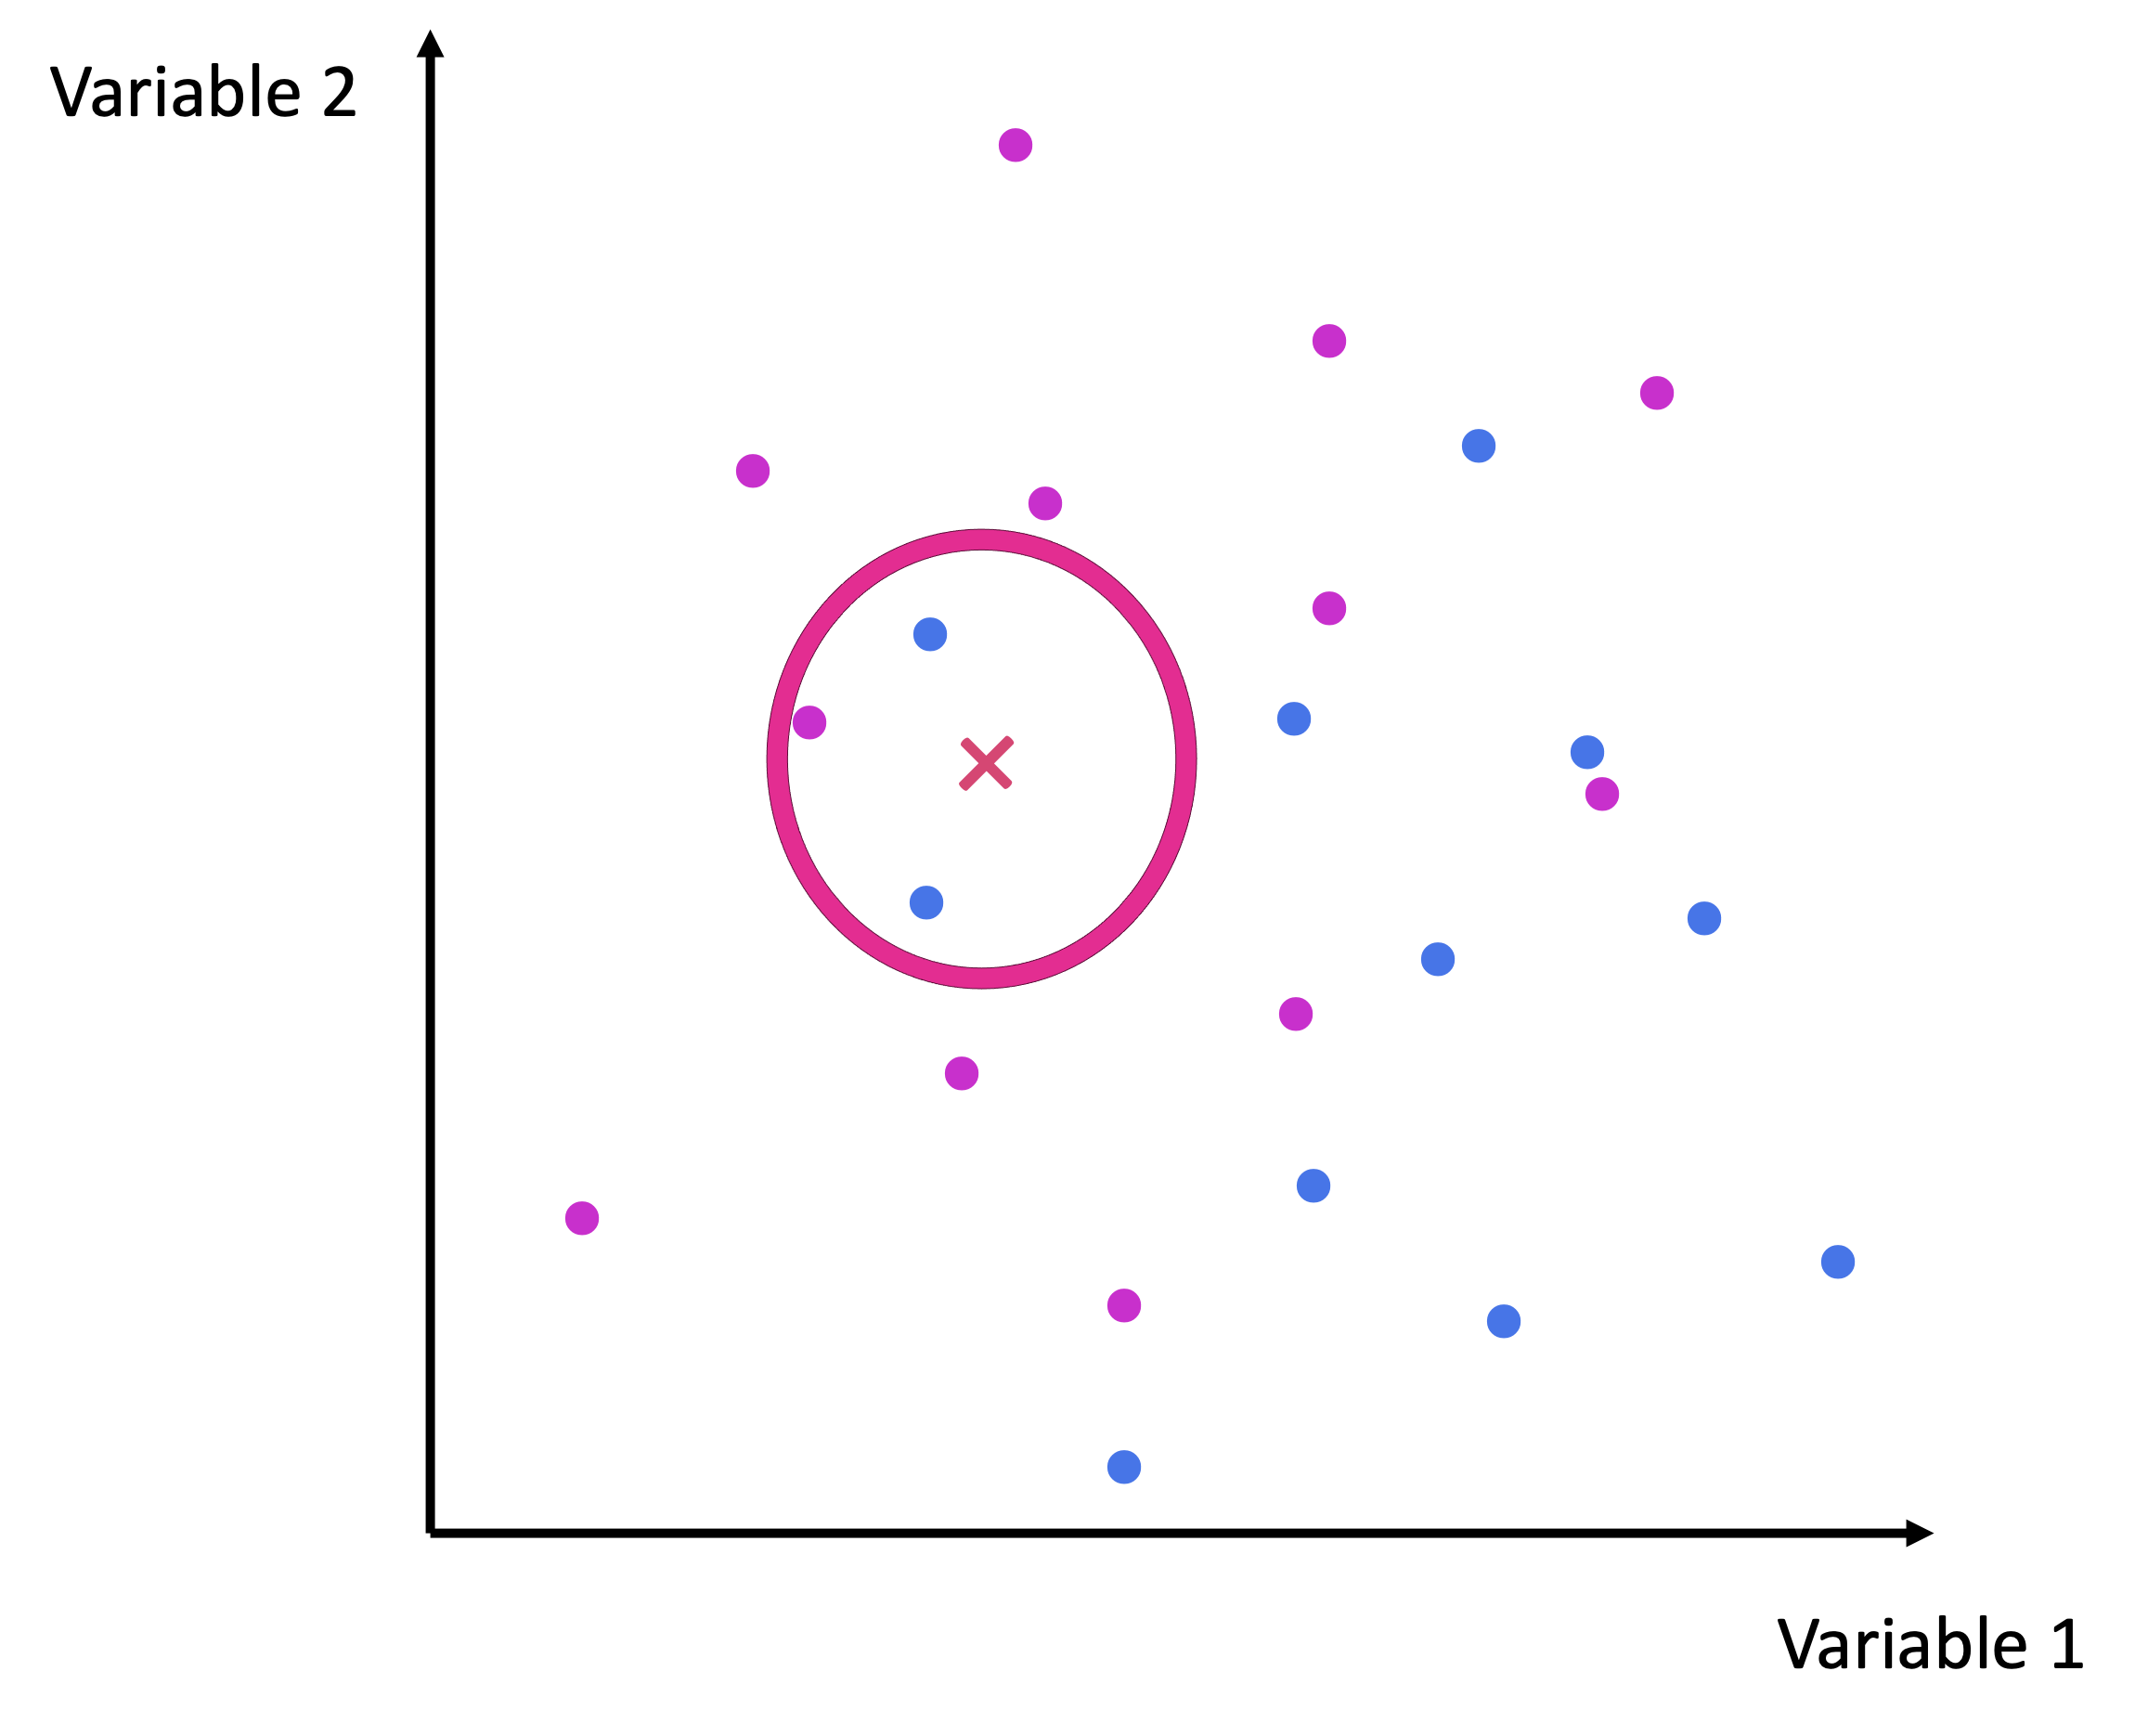
\includegraphics[width=0.3\textwidth]{./ML__kNN.png}
    \caption{k-nearest Neighbour with k = 3}
    \label{fig:ml_neurnet}
\end{figure}